\documentclass[letter,12pt]{article}
\usepackage[paperheight=27.94cm,paperwidth=21.59cm,bindingoffset=0in,left=3cm,right=2.0cm, top=3.5cm,bottom=2.5cm, headheight=200pt, headsep=1.0\baselineskip]{geometry}
\usepackage{graphicx,lastpage}
\usepackage{upgreek}
\usepackage{censor}
\usepackage[spanish,es-tabla]{babel}
\usepackage{pdfpages}
\usepackage{tabularx}
\usepackage{graphicx}
\usepackage{adjustbox}
\usepackage{xcolor}
\usepackage{colortbl}
\usepackage{rotating}
\usepackage{multirow}
\usepackage[utf8]{inputenc}
\usepackage{float}
\usepackage{hyperref}

\renewcommand{\tablename}{Tabla}
\usepackage{fancyhdr}
\pagestyle{fancy}

\usepackage{listing}
\usepackage{lstautogobble}
% Inline Code
\newcommand{\code}[1]{\colorbox{lightgray!80}{\lstinline[breaklines=true]|#1|}}
\newcommand{\BashCode}{
    \lstset{
        language=bash,
        basicstyle=\ttfamily\small,
        backgroundcolor=\color{lightgray!30},
        breaklines=true,
        showspaces=false,
        showstringspaces=false,
        numbers=left,
        % listings no tiene definido utf-8 por defecto
        % definimos cada carácter especial
        literate=
          {á}{{\'a}}1
          {é}{{\'e}}1
          {í}{{\'\i}}1
          {ó}{{\'o}}1
          {ú}{{\'u}}1
          {ñ}{{\~n}}1
          {¡}{{!`}}1
          {¿}{{?`}}1
      }
}

%
\begin{document}
%
   \title{\Huge{Informe Laboratorio 5}}

   \author{\textbf{Sección x} \\  \\Alumno x \\ e-mail: alumno.contacto@mail.udp.cl}
          
   \date{Junio de 2023}

   \maketitle
   
   \tableofcontents
 
  \newpage
  

\section{Descripción de actividades}
Para este último laboratorio, nuestro informante ya sabe que puede establecer un medio seguro sin un intercambio previo de una contraseña, gracias al protocolo diffie-hellman. El problema es que ahora no sabe si confiar en el equipo con el cual establezca comunicación, ya que las credenciales de usuario pueden haber sido divulgadas por algún soplón.\\

Para el presente laboratorio deberá:

\begin{itemize}
    \item Crear 4 contenedores en Docker, donde cada uno tendrá el siguiente SO:
        Ubuntu 14.10, Ubuntu 16.10, Ubuntu 18.10 y Ubuntu 20.10, a los cuales llamaremos C1,C2,C3,C4/S1 respectivamente.
        
    \item Para cada uno de ellos, deberá instalar la última versión, disponible en sus repositorios, del cliente y servidor openssh.

    \item En S1 deberá crear el usuario test con contraseña test, para acceder a él desde los otros contenedores.
    
    \item En total serán 4 escenarios, donde cada uno corresponderá a los siguientes equipos:
    \begin{itemize}
        \item C1 $\rightarrow$ S1
        \item C2 $\rightarrow$ S1
        \item C3 $\rightarrow$ S1
        \item C4 $\rightarrow$ S1
    \end{itemize}
\end{itemize}

Pasos:

\begin{enumerate}
\item Para cada uno de los 4 escenarios, solo deberá establecer la conexión y no realizar ningún otro comando que pueda generar tráfico (como muestra la Figura). Deberá capturar el tráfico de red generado y analizar el patrón de tráfico generado por cada cliente. De esta forma podrá obtener una huella digital para cada cliente a partir de su tráfico.\\

Indique el tamaño de los paquetes del flujo generados por el cliente y el contenido asociado a cada uno de ellos. Luego, indique qué información distinta contiene el escenario siguiente (diff incremental). El objetivo de esta tarea es identificar claramente los cambios entre las distintas versiones de ssh.

\newpage

\item Para poder identificar que el usuario efectivamente es el informante, éste utilizará una versión única de cliente. ¿Con qué cliente SSH se habrá generado el siguiente tráfico?

\begin{figure}[H]
    \centering
    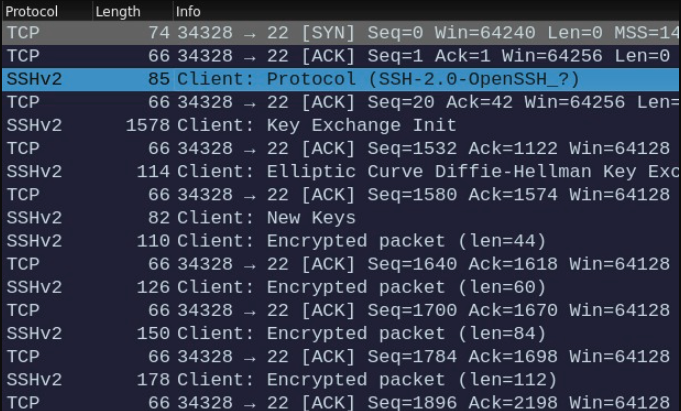
\includegraphics[width=17.5cm]{Desarrollo/trafico.png}
    \caption{Tráfico generado del informante}
    \label{fig:ASCII}
\end{figure}

Replique este tráfico generado en la imagen. Debe generar el tráfico con la misma versión resaltada en azul.

\newpage

\item Para que el informante esté seguro de nuestra identidad, nos pide que el patrón del tráfico de nuestro server también sea modificado, hasta que el Key Exchange Init del server sea menor a 300 bytes. Indique qué pasos realizó para lograr esto.

\begin{figure}[H]
    \centering
    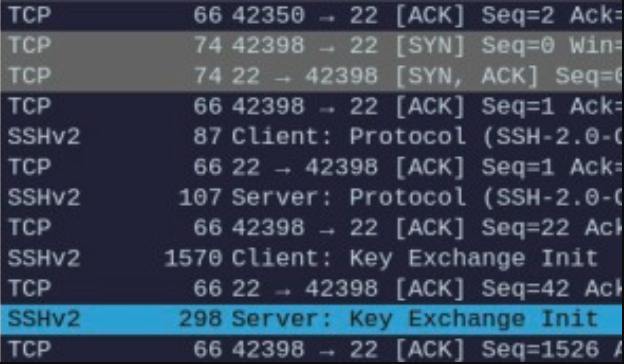
\includegraphics[width=17.5cm]{Desarrollo/exchange.png}
    \caption{Captura del Key Exchange}
    \label{fig:ASCII}
\end{figure}

\end{enumerate}


\newpage
\section{Desarrollo (Parte 1)}

\subsection{Códigos de cada Dockerfile}
Todos los contenedores se encuentran en versiones de Ubuntu en el estado End of Life (sin soporte activo). Es por esto que los repositorios dde archive.ubuntu.com y security.ubuntu.com para estas versiones no se encuentran disponibles, es por esto que remplazamos ambas URL por old-releases.ubuntu.com, además de esto, los 3 primeros contenedores consisten únicamente de un cliente SSH mientras que el cuarto es el único que también cumple rol de servidor SSH.
\subsubsection{C1}
\begin{listing}
    \BashCode{}
  \begin{lstlisting}
FROM ubuntu:14.10

# Use old-releases.ubuntu.com instead of archive.ubuntu.com or security.ubuntu.com
RUN sed -i -re 's/([a-z]{2}\.)?archive.ubuntu.com|security.ubuntu.com/old-releases.ubuntu.com/g' /etc/apt/sources.list

RUN apt-get update
RUN apt-get install -y openssh-client
  \end{lstlisting}
\end{listing}
\subsubsection{C2}
\begin{listing}
    \BashCode{}
  \begin{lstlisting}
FROM ubuntu:16.10

# Use old-releases.ubuntu.com instead of archive.ubuntu.com or security.ubuntu.com
RUN sed -i -re 's/([a-z]{2}\.)?archive.ubuntu.com|security.ubuntu.com/old-releases.ubuntu.com/g' /etc/apt/sources.list

RUN apt-get update
RUN apt-get install -y openssh-client
  \end{lstlisting}
\end{listing}
\subsubsection{C3}
\begin{listing}
    \BashCode{}
  \begin{lstlisting}
FROM ubuntu:18.10

# Use old-releases.ubuntu.com instead of archive.ubuntu.com or security.ubuntu.com
RUN sed -i -re 's/([a-z]{2}\.)?archive.ubuntu.com|security.ubuntu.com/old-releases.ubuntu.com/g' /etc/apt/sources.list

RUN apt-get update
RUN apt-get install -y openssh-client
  \end{lstlisting}
\end{listing}
\subsubsection{C4/S1}
\begin{listing}
    \BashCode{}
  \begin{lstlisting}
FROM ubuntu:20.10

# Use old-releases.ubuntu.com instead of archive.ubuntu.com or security.ubuntu.com
RUN sed -i -re 's/([a-z]{2}\.)?archive.ubuntu.com|security.ubuntu.com/old-releases.ubuntu.com/g' /etc/apt/sources.list

RUN apt-get update
RUN apt-get install -y \
    openssh-client \
    openssh-server

# Create "test" user
RUN useradd -m -s /bin/bash test
# Create password for test user, password: test
RUN echo "test:test" | chpasswd

# Expose port 22 for SSH connection
EXPOSE 22

ENTRYPOINT service ssh restart && bash
  \end{lstlisting}
\end{listing}

\subsection{Creación de las credenciales para S1}
Para la creación de credenciales se necesita un usuario y definir una contraseña para el mismo. Esto se logra con los siguientes comandos.

\begin{listing}
    \BashCode{}
  \begin{lstlisting}
# Create "test" user
RUN useradd -m -s /bin/bash test
# Create password for test user, password: test
RUN echo "test:test" | chpasswd
  \end{lstlisting}
\end{listing}

\subsection{Tráfico generado por C1 (detallado)}
En todas las capturas de tráfico el protocolo SSH funciona sobre TCP, por lo que contiene un handshake y un ACK en cada paso del protocolo SSH. Por simplicidad se usa el filtro SSH en Wireshark para todas las capturas.

\begin{figure}[H]
  \centering
  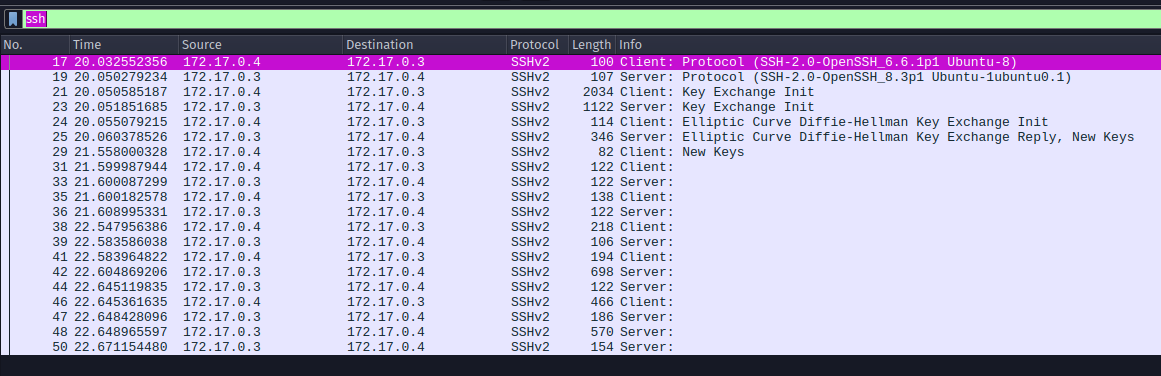
\includegraphics[width=16cm]{Images/01-capture-c1-to-c4.png}
  \caption{Captura c1 (Ubuntu 14.10) a s1 (Ubuntu 20.10).}
\end{figure}

Desde la captura se puede desprender la versión de OpenSSH del cliente (v6.6.1) y del servidor (v8.3). El protocolo se puede conocer en el intercambio de llaves, en este caso el protocolo utilizado es Diffie-Hellman. Y luego, 13 mensajes cifrados de distintos tamaños.

\subsection{Tráfico generado por C2 (detallado)}
\begin{figure}[H]
  \centering
  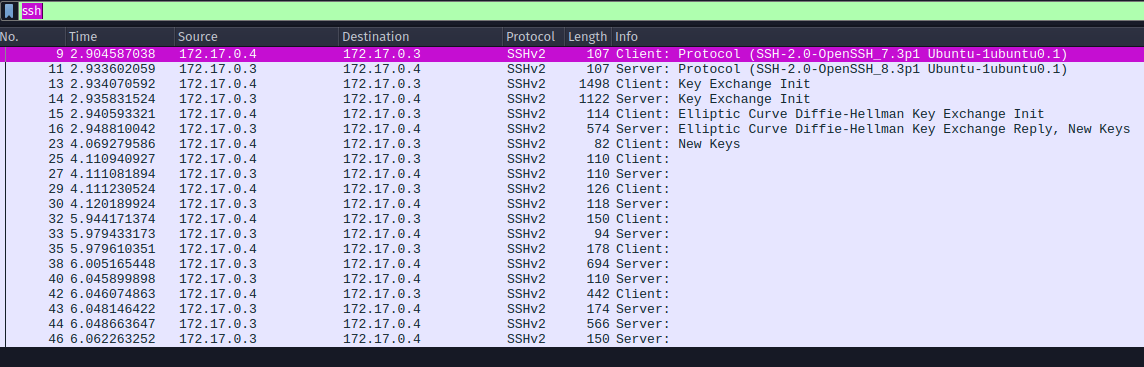
\includegraphics[width=16cm]{Images/02-capture-c2-to-c4.png}
  \caption{Captura c2 (Ubuntu 16.10) a s1 (Ubuntu 20.10).}
\end{figure}

De la captura se desprende la versión de OpenSSH del cliente (v.7.3) y del servidor (v8.3). Utilizan el mismo protocolo que la captura anterior (Diffie-Hellman). Igualmente termina con 13 mensajes cifrados de distintos tamaños.

\subsection{Tráfico generado por C3 (detallado)}
\begin{figure}[H]
  \centering
  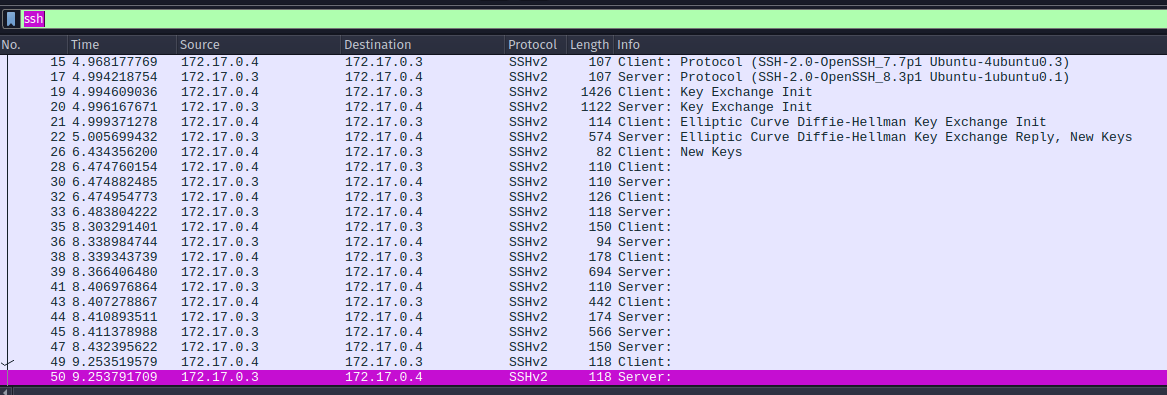
\includegraphics[width=16cm]{Images/03-capture-c3-to-c4.png}
  \caption{Captura c3 (Ubuntu 18.10) a s1 (Ubuntu 20.10).}
\end{figure}

De la captura se desprende la versión de OpenSSH del cliente (v.7.7) y del servidor (v8.3). Utilizan el mismo protocolo que la captura anterior (Diffie-Hellman). Termina con 14 mensajes cifrados de distintos tamaños.

\subsection{Tráfico generado por C4 (iface lo) (detallado)}

\begin{figure}[H]
  \centering
  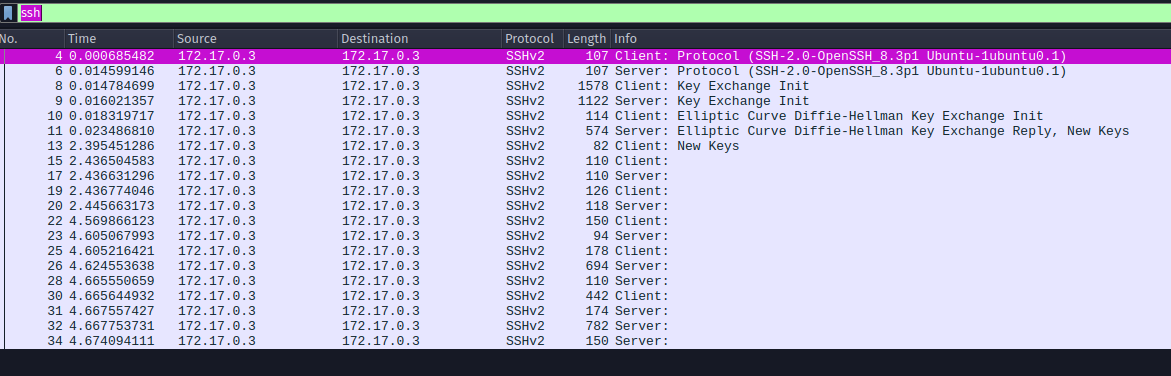
\includegraphics[width=16cm]{Images/04-capture-c4-to-c4.png}
  \caption{Captura c4 (Ubuntu 20.10) a s1 (Ubuntu 20.10).}
\end{figure}

De la captura se puede desprender que el cliente y el servidor corresponden al mismo host, ya que, la IP de fuente y de destino es la misma (172.17.0.3) como también, se puede conocer la versión de OpenSSH (v8.3). Se puede notar que aunque el cliente y el servidor se encuentran en el mismos host se realiza el protocolo completo de SSH, es decir, el intercambio de llaves y luego 13 mensajes encriptados.

\subsection{Diferencia entre C1 y C2}
Entre C1 y C2 existe un salto de versión mayor (de v6.x a v7.x). Ambos contienen la misma serie de pasos: Anuncian su versión, ambos inician el intercambio de llaves, definen un protocolo para enviarla y finalmente el cliente anuncia que tiene una nueva llave; terminan con 13 mensajes cifrados. La única diferencia son los tamaños de los paquetes en cada uno de estos paso excepto la señal ``Client: New Keys''.

\subsection{Diferencia entre C2 y C3}
Entre C2 y C3 no existe un salto de versión mayor (de v7.3 a v7.7) y en general, todos los paquetes tienen un mismo tamaño excepto el ``Client: Key Exchange Init'', además, C3 envía 1 mensaje cifrado más con respecto a C2 (también con respecto a C1 y C4). Esto puede ser circunstancial o no, no se puede inspeccionar el paquete ya que está encriptado.

\subsection{Diferencia entre C3 y C4}
Entre C3 y C4 sí existe un salto de versión mayor (de v7.7 a v8.3). Siguen invariantes los pasos del protocolo, vuelve a variar el tamaño de los paquetes.

\section{Desarrollo (Parte 2)}
\subsection{Identificación del cliente ssh}
Desde la imagen se puede notar que el ``Client: Key Exchange Init'' tiene exactamente 1578 Bytes. La única versión que coincide con esto es la captura c4 a c4 con OpenSSH v8.3.

\begin{itemize}
        \item C1 a C4 tiene un ``Client: Key Exchange Init'' de tamaño 2034 bytes.
        \item C2 a C4 tiene un ``Client: Key Exchange Init'' de tamaño 1498 bytes.
        \item C3 a C4 tiene un ``Client: Key Exchange Init'' de tamaño 1498 bytes.
        \item C4 a C4 tiene un ``Client: Key Exchange Init'' de tamaño 2034 bytes.
\end{itemize}

Cabe destacar, que desde estos datos se puede intuir que entre versiones mayores se mantienen los tamaños de los mensajes del protocolo SSH.

\subsection{Replicación de tráfico (paso por paso)}

Para replicar el tráfico se puede compilar desde fuente, para esto se necesita un compilador, una librería para compresión (zlib) y una librería para encriptación (libssl). Antes de compilar basta con modificar el archivo version.h y colocar el string deseado, en este caso \text{OpenSSH\_?}. A continuación el Dockerfile que genera este contenedor (cliente-modificado):

\begin{listing}
    \BashCode{}
  \begin{lstlisting}
FROM ubuntu:20.10

# Use old-releases.ubuntu.com instead of archive.ubuntu.com or security.ubuntu.com
RUN sed -i -re 's/([a-z]{2}\.)?archive.ubuntu.com|security.ubuntu.com/old-releases.ubuntu.com/g' /etc/apt/sources.list

RUN apt-get update
RUN apt-get install -y \
    git \
    autoconf \
    gcc \
    zlib1g-dev \
    libssl-dev \
    make \
    wget

RUN wget https://cdn.openbsd.org/pub/OpenBSD/OpenSSH/portable/openssh-8.3p1.tar.gz
RUN tar zxvf openssh-8.3p1.tar.gz
WORKDIR /openssh-8.3p1
RUN sed -i 's/8.3/?/' version.h

RUN ./configure
RUN make
RUN make install
  \end{lstlisting}
\end{listing}

Generamos el tráfico y comprobamos:
\begin{figure}[H]
  \centering
  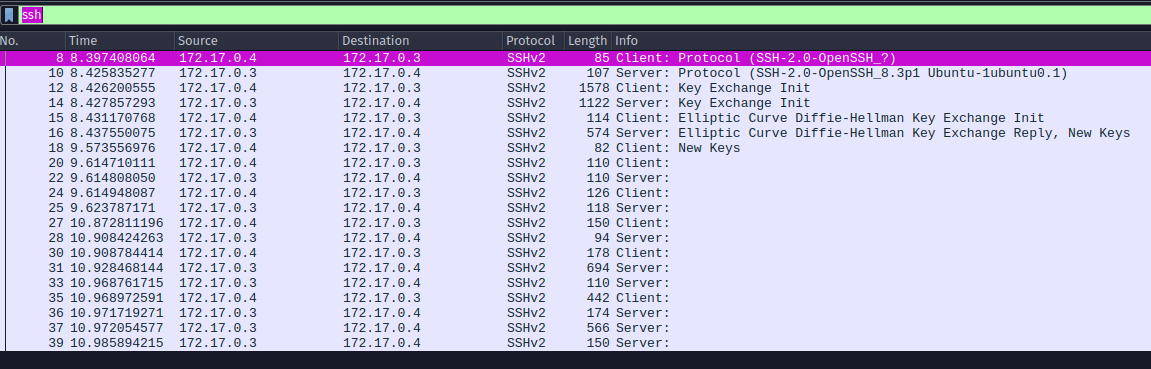
\includegraphics[width=16cm]{Images/05-capture-modified-client.png}
  \caption{Captura cliente-modificado (Ubuntu 20.10) a s1 (Ubuntu 20.10).}
\end{figure}

\section{Desarrollo (Parte 3)}
\subsection{Replicación de tráfico (paso por paso)}
Gran parte del payload del paquete SSH que envía el servidor hacia el cliente es información sobre los protocolos y cifrados disponibles. Se puede acortar el tamaño del archivo especificando un único parámetro válido. Se genera un Dockerfile llamado ``server-modificado'' con los sigiuentes cambios:

\begin{listing}
    \BashCode{}
  \begin{lstlisting}
RUN echo "HostKey /etc/ssh/ssh_host_ecdsa_key" >> /etc/ssh/sshd_config
RUN echo "KexAlgorithms diffie-hellman-group-exchange-sha256" >> /etc/ssh/sshd_config
RUN echo "MACs hmac-sha2-512" >> /etc/ssh/sshd_config
RUN echo "Ciphers aes256-ctr" >> /etc/ssh/sshd_config
  \end{lstlisting}
\end{listing}

El servidor SSH ya parte con las condiciones necesarias y se captura el tráfico.
\begin{figure}[H]
  \centering
  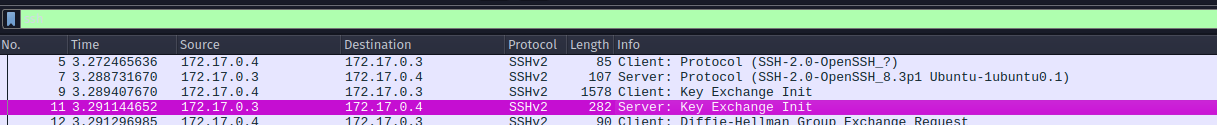
\includegraphics[width=16cm]{Images/06-capture-modified-server.png}
  \caption{Captura server-modificado con tamaño de paquete reducido.}
\end{figure}

\section*{Conclusiones y comentarios}
En el paso informe se puede ver cómo se puede transmitir información de manera sutil manejando las diferencias coom versiones de un mismo software que contiene variaciones difíciles de notar. Además se ve cómo esto se puede lograr tanto como del lado del cliente como del servidor.

\end{document}
